\documentclass[10pt, margin=1mm]{standalone}
\usepackage{tikz}
\usetikzlibrary{arrows,decorations.pathmorphing,backgrounds,positioning,fit,petri,shapes}
\pgfdeclarelayer{bg}    % declare background layer
\pgfsetlayers{bg,main}  % set the order of the layers (main is the standard layer)
\usepackage{graphicx}
\usepackage{amsmath,amssymb,amsfonts}
\usepackage{fontawesome}

\definecolor{myblue}{RGB}{76,114,176}
\definecolor{myorange}{RGB}{221,132,82}

\usetikzlibrary{shapes.multipart}

\begin{document}
    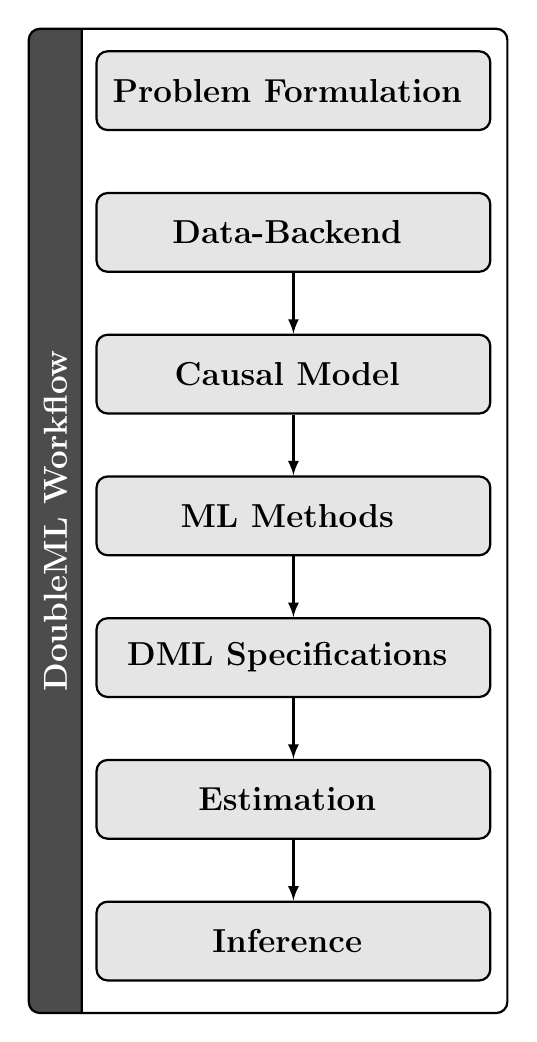
\begin{tikzpicture}[scale=0.9]
%[auto,scale=1,transition/.style={rectangle,draw=black!50,thick,
%inner sep=5pt,minimum width=8cm,minimum height=1cm,font=\large,text width=8cm}]
\tikzstyle{every node}=[font=\large\bf]

\node[rotate=90,thick,below,
minimum width=12.5cm,
rectangle split,rectangle split parts=2, inner sep=5pt, rounded corners, draw=black,
rectangle split part align={center, left},
rectangle split part fill={black!70, white}] at (-3.75, -3.5) (doubleml) {
\textcolor{white}{
DoubleML Workflow}
\nodepart{two}{%
\begin{tabular}{l}
\\ \\ \\ \\ \\ \\ \\ \\ \\ \\[3pt]
\end{tabular}
}
};


%\node[anchor=north, thick,above, fill=black!70, align=center,
%rectangle, inner sep=5pt, rounded corners, draw=black] at (0, 0) (s3) {
%\textcolor{white}{Data-Backend}
%};

\node[anchor=north, thick,above, fill=black!10, align=center,
minimum width=5cm, minimum height=1cm,
rectangle, inner sep=5pt, rounded corners, draw=black] at (0, 2) (problem) {
Problem Formulation
};

\node[anchor=north, thick,above, fill=black!10, align=center,
minimum width=5cm, minimum height=1cm,
rectangle, inner sep=5pt, rounded corners, draw=black] at (0, 0) (data) {
Data-Backend
};

\node[anchor=north, thick,above, fill=black!10, align=center,
minimum width=5cm, minimum height=1cm,
rectangle, inner sep=5pt, rounded corners, draw=black] at (0, -2) (causal) {
Causal Model
};

\node[anchor=north, thick,above, fill=black!10, align=center,
minimum width=5cm, minimum height=1cm,
rectangle, inner sep=5pt, rounded corners, draw=black] at (0, -4) (ml) {
ML Methods
};

\node[anchor=north, thick,above, fill=black!10, align=center,
minimum width=5cm, minimum height=1cm,
rectangle, inner sep=5pt, rounded corners, draw=black] at (0, -6) (dml) {
DML Specifications
};

\node[anchor=north, thick,above, fill=black!10, align=center,
minimum width=5cm, minimum height=1cm,
rectangle, inner sep=5pt, rounded corners, draw=black] at (0, -8) (est) {
Estimation
};

\node[anchor=north, thick,above, fill=black!10, align=center,
minimum width=5cm, minimum height=1cm,
rectangle, inner sep=5pt, rounded corners, draw=black] at (0, -10) (inf) {
Inference
};

\draw[-latex, thick] (data.south) -- (causal.north);
\draw[-latex, thick] (causal.south) -- (ml.north);
\draw[-latex, thick] (ml.south) -- (dml.north);
\draw[-latex, thick] (dml.south) -- (est.north);
\draw[-latex, thick] (est.south) -- (inf.north);

\end{tikzpicture}

\end{document}
